\section{Theoretical Analysis}
\label{sec:analysis}
\indent

In this section, the circuit shown in Figure~\ref{fig:rc} is analysed
theoretically, using the mesh and the node methods. 

\subsection{Mesh analysis}
%imagem
\begin{figure}[H] \centering
    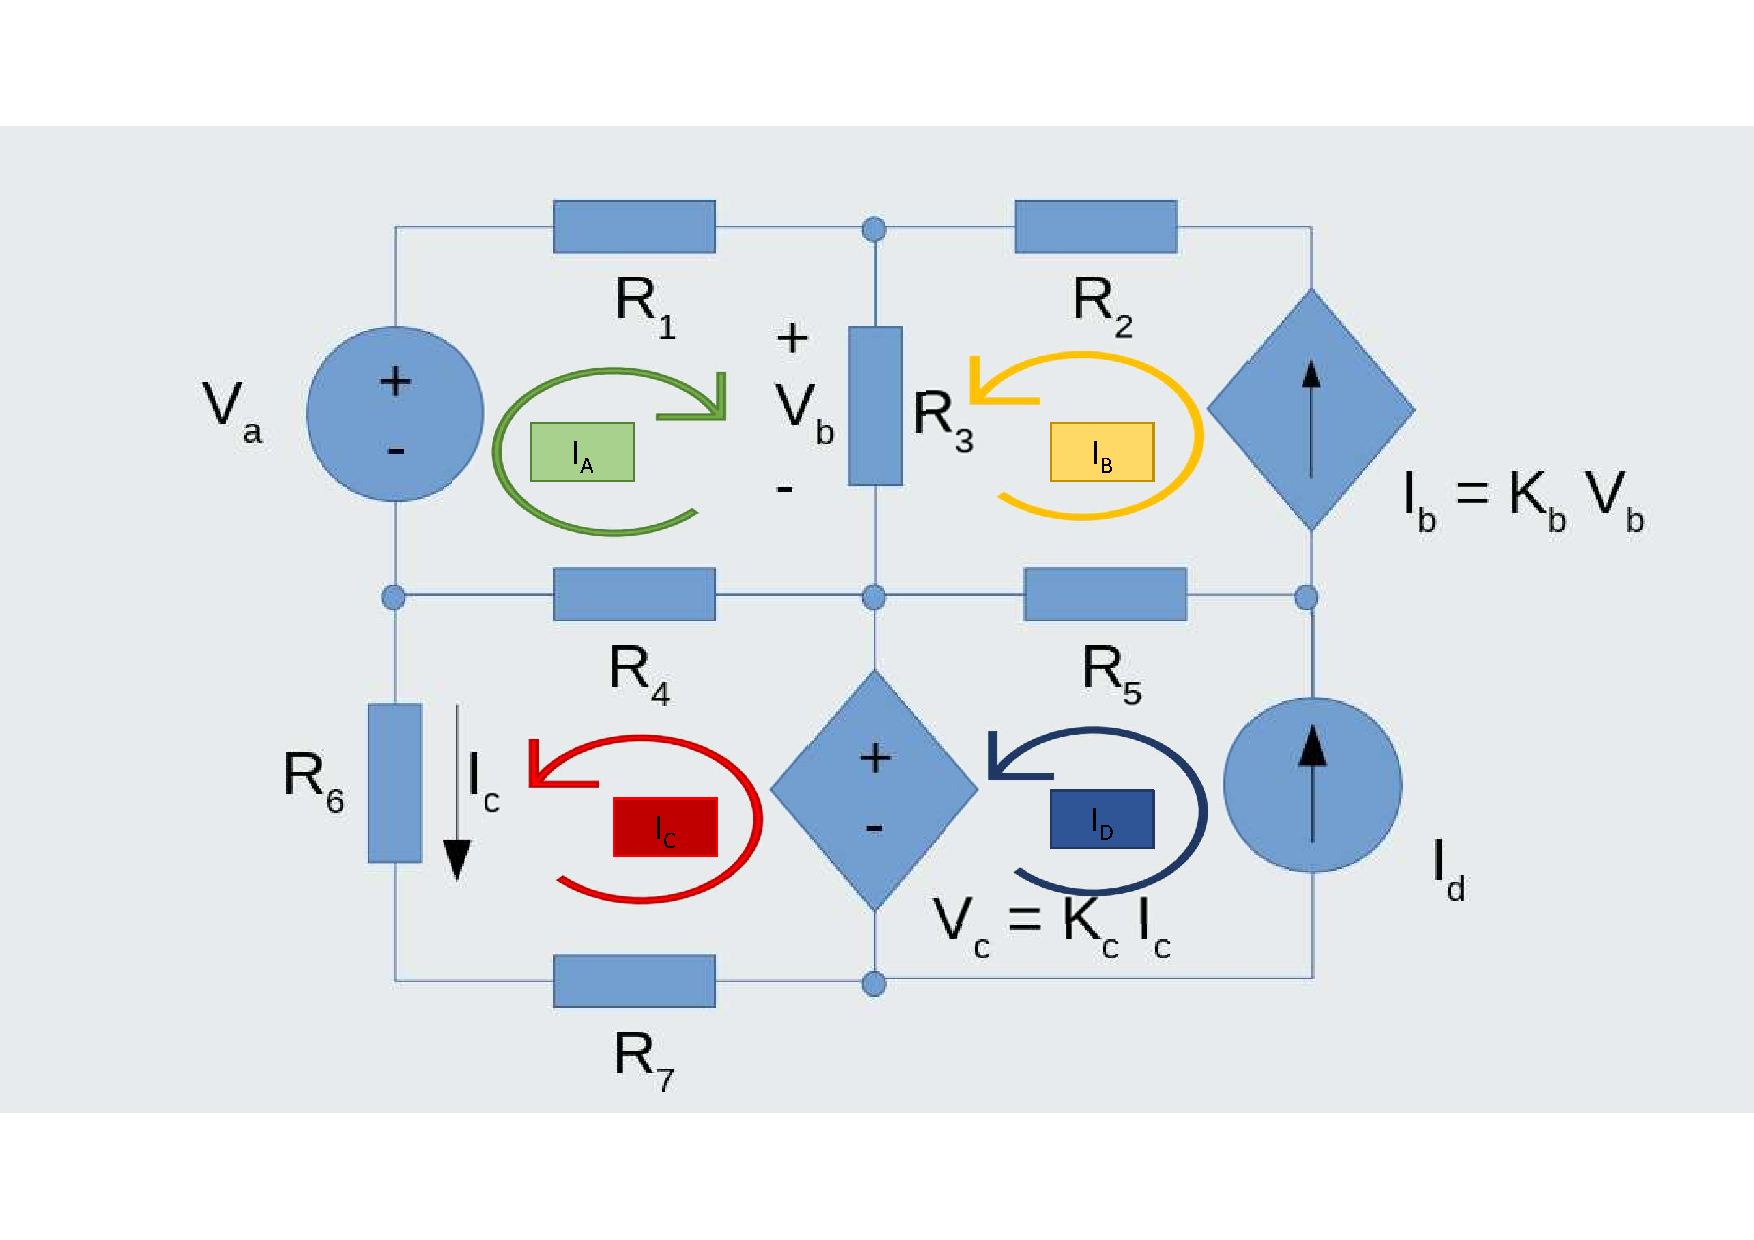
\includegraphics[width=0.8\linewidth]{Images/mesh analysis.pdf}
    \caption{Current flow by mesh.}
    \label{fig:Currents}
\end{figure}


\indent

This circuit is composed by four primary meshes in which we assume the current flows counter-clockwise in every mesh but one, as seen in Figure~\ref{fig:Currents}.

Note that this is merely a convention used in our theoretical computations. The actual physical direction of the current can be obtained by analysing the algebraic sign of the current in each branch. 

To find out the current that flows in each mesh we use the Kirchhoff Voltage Law (KVL) followed by Ohm's Law. 

\begin{equation}
    \sum_{k=1}^{n} V_k = 0.
    \quad\text{,}\quad 
    V=RI.
\end{equation}

In some cases, two currents flow on the same branch. To solve this we use  Kirchhoff Current Law (KCL), to find the current on that branch.

\begin{equation}
    \sum_{k=1}^{n} I_k = 0.
    \label{eq:KCL}
\end{equation}

In mesh $a$ (mesh where the current $I_a$ flows) we assume that the voltage source is providing energy to the circuit and therefore the current has to flow clock-wise. This means that the sum of the voltages in each resistor ($R_1$, $R_3$ and $R_4$) has to equal the voltage $V_a$.

In meshes $b$, $c$ and $d$ we followed the same process as in mesh $a$, defining the way in which the current flows through current and voltage sources.
To exemplify this process, the equation for mesh $a$ is the following:

\begin{equation}
    V_a=R_1I_a+R_3(I_a+I_b)+R_4(I_a+I_c).
\end{equation}

With the aid of octave, we can solve the four equations to obtain the following table (table~\ref{tab:Imesh}).

\begin{table}[h]
  \centering
  \begin{tabular}{|l|r|}
    \hline    
    {\bf Name} & {\bf Value [mA]} \\ \hline
    Ia & 0.194523 \\ \hline 
Ib & -0.204136 \\ \hline 
Ic & 0.961761 \\ \hline 
Id & 0.000000 \\ \hline 

  \end{tabular}
  \caption{Results from the mesh analysis, from \textit{Octave}.}
  \label{tab:Imesh}
\end{table}

Since we know the current on each mesh we can calculate the current on every branch. The results are present on table~\ref{tab:Ibranch}.

\begin{table}[h]
  \centering
  \begin{tabular}{|l|r|}
    \hline    
    {\bf Name} & {\bf Value [mA]} \\ \hline
    Ib & -0.204136 \\ \hline 
Id & 0.000000 \\ \hline 
R1 & 0.194523 \\ \hline 
R2 & -0.204136 \\ \hline 
R3 & -0.009613 \\ \hline 
R4 & 1.156284 \\ \hline 
R5 & 0.204136 \\ \hline 
R6 & 0.961761 \\ \hline 
R7 & 0.961761 \\ \hline 

  \end{tabular}
  \caption{Current on each branch.}
  \label{tab:Ibranch}
\end{table}


\subsection{Node analysis}

\begin{figure}[H] \centering
    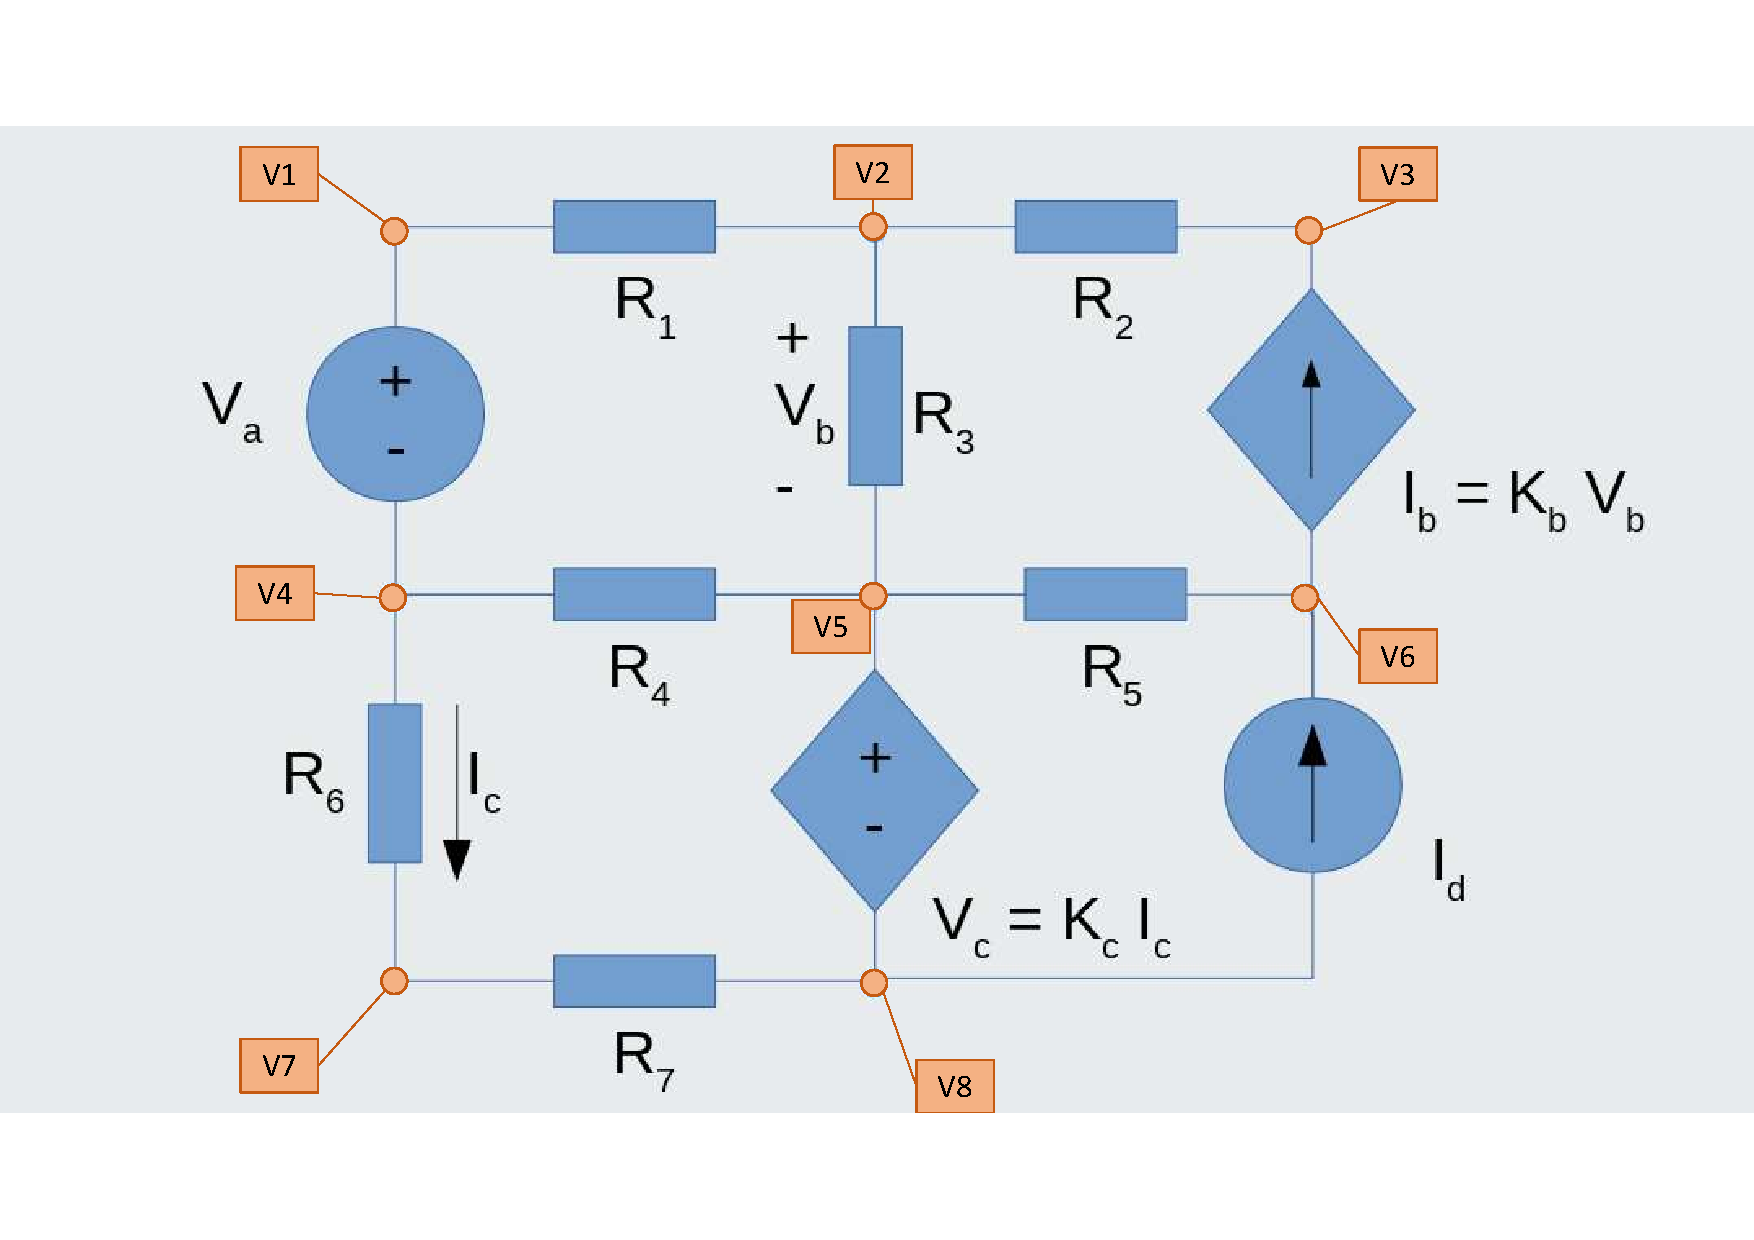
\includegraphics[width=0.8\linewidth]{Images/node analysis.pdf}
    \caption{Nodes.}
    \label{fig:Nodes}
\end{figure}

\indent

There are 8 nodes in total which means that we need 8 equations to find out the voltages in each node and solve the circuit. Therefore, we use the Kirchhoff Current Law (KCL, equation~\ref{eq:KCL}) in every node that is not connected to a voltage source (nodes 2, 3, 6 and 7, which are identified in Figure~\ref{fig:Nodes} ).

We assume node 4 ($V_4$) as the reference node, which means that its value is 0. This node was chosen because usually, the negative terminal of a voltage source is connected to the ground.

It is also known that the value of a voltage source is equivalent to the difference of the voltages in each node to which the source is connected. That allows us to create two more equations, since there are two voltage sources in the circuit.

For the $8^{th}$ equation we can create a supernode with nodes 5 and 8 since the dependent voltage source is not connected to the reference node. This way, nodes 5 and 8 are considered as one by ignoring the voltage source between them.

To demonstrate the process, the node 2 equation resulting from the KCL application is the following:

\begin{equation}
    (V_2-V_3)G_2=(V_5-V_2)G_3+(V_1-V_2)G_1.
\end{equation}

Doing this on all possible nodes/supernode and adding the extra equations, regarding the voltage sources, a system of linear equations can be obtained and solved with the aid of \textit{Octave}. The results are presented on table~\ref{tab:Volts}.

\begin{table}[h]
  \centering
  \begin{tabular}{|l|r|}
    \hline    
    {\bf Name} & {\bf Value [V]} \\ \hline
    V1 & 5.008942 \\ \hline 
V2 & 4.808960 \\ \hline 
V3 & 4.394159 \\ \hline 
V4 & 0.000000 \\ \hline 
V5 & 4.837862 \\ \hline 
V6 & 5.474755 \\ \hline 
V7 & -2.008723 \\ \hline 
V8 & -2.970917 \\ \hline 

  \end{tabular}
  \caption{Results from the node analysis, from \textit{Octave}.}
  \label{tab:Volts}
\end{table}
